\documentclass[english,a4paper]{article}
\usepackage[latin1]{inputenc}
\usepackage{babel}
\usepackage{listings}
\usepackage{float}
\usepackage{type1cm}
\usepackage{paralist}
\usepackage{graphicx}
\usepackage{amssymb}
\usepackage[hyphens]{url}

\floatstyle{boxed}
\restylefloat{figure}
\setcounter{topnumber}{5}
\setcounter{bottomnumber}{5}
\setcounter{totalnumber}{10}
\renewcommand{\topfraction}{0.9}
\renewcommand{\bottomfraction}{0.9}
\renewcommand{\textfraction}{0.1}
\renewcommand{\floatpagefraction}{0.9}

\newfloat{Listing}{tbp}{pro}

\lstset{language=C++,
  columns=fullflexible,
  basicstyle=\sffamily,
  commentstyle=\itshape}

% This command does two things:
% #1 ensure that non-keywords are printed non-bold, even in titles.
% #2 fold newlines into spaces before they are given to \lstinline so
%    I don't need to care where I break my lines in normal text.
\newcommand{\code}[1]{\textnormal{\lstinline{#1}}}

% don't use the dash in enumerations because it look too much like a
% minus
\setdefaultitem{\textbullet}{\textbullet}{\textbullet}{\textbullet}

\author{J.~Fahlke}
\title{Implementing Local and Temporary Refinements in Dune}
\date{6th February 2006}

%
% Structure of the document:
% - Introduction (What is Refinement, and what is its purpose)
% - Design of the Interface
%   - Refinement
%   - Why are the Iterators not dereferenceable
%   - VirtualRefinement
%   - buildRefinement()
% - Extending Refinement
% - Overview of the implementation
%   - hcube
%   - simplex (short)
%   - triangulation
% - Implementing Refinement of simplices
%   - Kuhn triangulation
%   - Refining simplices
%   - Terminology
%   - Kuhn simplex <-> permutation
%   - Permutation <-> Integer
%   - Counting vertices
%   - Numbering vertices
%   - Counting Elements
%   - Numbering Elements
%   - Transformation reference <-> Kuhn simplex
%

\begin{document}
\maketitle

\section{Introduction}

Refinement is a subsystem of Dune\cite{dune} which allows for local
and temporary refinements of arbitrary grid entities without having to
modify the grid or the entity itself.  This allows to interpolate
nonlinear functions into linear pieces.

It can also be used to partition entities of one geometry type into
subentities of another geometry type, e.\,g.\ quadrilaterals into
triangles.  This is useful if we want to write a grid and associated
data into a file, but the file format can only deal with one geometry
type.

\section{Design of the Interface}

\subsection{Terminology}

\begin{description}
\item[Entity:] An entity is an arbitrary polytope which is a member of
  a grid.  It may have the same dimension as the grid itself or any
  lower dimension.
\item[Element:] An element is an {\em entity} of the same dimension as
  the grid it belongs to.
\item[Vertex:] A vertex is an {\em entity} of dimension 0 (a point).
\item[Codimension:] Let $d_G$ be the dimension of a grid and $d_e$ the
  dimension of one of its {\em entities}.  The codimension $c_e$ of that
  entity is defined as $c_e:=d_G-d_e$.  That means that the
  codimension of a {\em vertex} equals the dimension of its grid,
  while the codimension of an {\em element} is alway 0.
\item[Subentity:] When we refine an {\em entity}, we can view it as a
  grid consisting of smaller entities of the same or lower dimension.
  To distinguish these smaller entities from those who belong to a
  full-fledged grid, we call then subentities.  Subentities also have
  a codimension: let $d_e$ be the dimension of the refined entity and
  $d_s$ be the dimension of one of its subentities, than $c_s:=d_e-d_s$
  is the codimension of the subentity.
\item[Subelement:] A subelement is a {\em subentity} with a
  codimension of 0.  It has the same dimension as the {\em entity} it
  refines.
\item[Subvertex:] A subvertex is a {\em subentity} with a dimension of
  0.  Its codimension equals the dimension of the {\em entity} it
  refines.
\end{description}

The prefix ``sub-'' may be omitted when it is clear that we are
talking about subentities instead of entities.

\subsection{General Considerations}

What data do we need to refine an entity, and what data do we want
back?

We want the subelements.  That means: how many subelements are
there, what are their indices within the refined entity, and what are
their corners.  That leads to the next topic: we want the subvertices.
That means: how many subvertices are there, and what are their indices
and positions within the refined entity.

To get this data, we need the geometry type of the entity we want to
refine and the geometry type of the entities we want back.  Of course,
we need the dimension of the entities as well.  We will do the
refining on Dunes reference elements, so this is all the information
we need about the entity to be refined.  Finally, we need to know the
refinement level, that is, how fine the subentities should be.

There is one addition: each grid in Dune may have its own C++ type for
its coordinates.  We pass that to Refinement as well, so it can do the
calculation with the same precision as the grid itself.

\begin{Listing}
  \begin{lstlisting}{}
template<NewGeometryType::BasicType geometryType,
         class CoordType,
         NewGeometryType::BasicType coerceTo,
         int dimension>
class Refinement
{
public:
  enum { dimension };

  template<int codimension>
  struct Codim {
    class SubEntityIterator;
  };
  typedef Codim<dimension>::SubEntityIterator VertexIterator;
  typedef Codim<0>::SubEntityIterator ElementIterator;

  typedef FieldVector<int, nCorners> IndexVector;
  typedef FieldVector<CoordType, dimension> CoordVector;

  static int nVertices(int level);
  static VertexIterator vBegin(int level);
  static VertexIterator vEnd(int level);

  static int nElements(int level);
  static ElementIterator eBegin(int level);
  static ElementIterator eEnd(int level);
}
  \end{lstlisting}
  \caption{The interface of \code{class Refinement}.}
  \label{intf_stat}
\end{Listing}

\subsection{\code{class Refinement}}

We chose an interface somewhat similar to the grid interface in Dune,
so our users don't have to learn totally new concepts.  The
\code{class Refinement} has methods to count the number of subelements
and the number of vertices on a given refinement level.  It also
contains iterators which iterate over the subelements and subvertices
of the refinement.

But that is where the similarity ends.  There is no support for
subentities other than subelements and subvertices.  \code{class
  Refinement} needs no information about itself at runtime, so it
contains only static methods and we can't actually create instances of
it.

Listing \ref{intf_stat} shows the interface of \code{class
  Refinement}.  To make compiler optimisation possible, it gets the
geometry type and the dimension of the refined entity, the geometry
type of its subelements and the coordinate type as template
parameters.  The only runtime parameter is the refinement level.

\begin{Listing}
  \begin{lstlisting}{}
template<NewGeometryType::BasicType geometryType,
         class CoordType,
         NewGeometryType::BasicType coerceTo,
         int dimension>
class VertexIterator
{
public:
  typedef Refinement;

  int index() const;
  Refinement::CoordVector coords() const;
};

template<NewGeometryType::BasicType geometryType,
         class CoordType,
         NewGeometryType::BasicType coerceTo,
         int dimension>
class ElementIterator
{
public:
  typedef Refinement;

  int index() const;
  // This is a FieldVector for Refinements iterators
  // but a std::vector for VitualRefinements iterators
  Refinement::IndexVector vertexIndices() const;
}
  \end{lstlisting}
  \caption{\label{intf_iter}The interface for the iterators of
    \code{class Refinement} and \code{class} \code{VirtualRefinement}.
    In addition to what is shown here, these iterators can do all the
    usual things iterators can do, except dereferencing.}
\end{Listing}

\subsubsection{The Iterators}

We decided to deviate from the usual scheme of an iterator in one
respect: the iterators are not dereferenceable.  Instead, you get the
information by directly calling methods of the iterator (see listing
\ref{intf_iter}).  The reason is that the subentities do not actually
exist as data within the grid; everything can be calculated on the fly
while incrementing the iterator.  The solution to maintain an entity
object within the iterator and return a reference to that is
non-satisfactory, since we have no control over the lifetime of that
reference.

\begin{Listing}
  \begin{lstlisting}{}
template<int dimension, class CoordType>
class VirtualRefinement
{
public:
  template<int codimension>
  struct Codim {
    class SubEntityIterator;
  };
  typedef Codim<dimension>::SubEntityIterator VertexIterator;
  typedef Codim<0>::SubEntityIterator ElementIterator;

  typedef std::vector<int> IndexVector;
  typedef FieldVector<CoordType, dimension> CoordVector;

  virtual int nVertices(int level) const;
  VertexIterator vBegin(int level) const;
  VertexIterator vEnd(int level) const;
  virtual int nElements(int level) const;
  ElementIterator eBegin(int level) const;
  ElementIterator eEnd(int level) const;
};
  \end{lstlisting}
  \caption{The interface of \code{class VirtualRefinement}.}
  \label{intf_virt}
\end{Listing}

\subsection{\code{class VirtualRefinement}}

\code{class Refinement} needs to know the geometry types of the
entities and subelements as compile time, which can make it cumbersome
to use if the grid which is refined contains elements of more than one
geometry type.  To make this easier we created \code{class
  VirtualRefinement} which defines the interface for a set of wrapper
classes.  Each wrapper provides the functionality of one corresponding
\code{class Refinement} with the interface of \code{class
  VirtualRefinement}.

The advantage is that our users can treat all \code{VirtualRefinement}
classes the same, so they only have to write their code once.  The
disadvantages are that the class is no longer static and it is now
decided at runtime which object is called, so the compiler cannot
inline these methods.  Of course, Refinement was developed with
disk-based input/output in mind, which is slow anyway, so there is not
much lost.

Listing \ref{intf_virt} shows the interface of \code{class
  VirtualRefinement}.  As can be seen it still has the template
parameters \code{class CoordType} and \code{int dimension}.  It does
not make sense to make the coordinate type selectable at runtime.  As
for the dimension: the user most probably knows it at compile time,
and it enables us to use fixed-size vectors for the coordinates.

\subsubsection{The Iterators}

The interface of the iterators (see listing \ref{intf_iter}) is the
same as for the iterators of \code{class} \code{Refinement}.  There is
one thing to note though: \code{class Refinement}s \code{IndexVector}
is an instance of Dunes \code{FieldVector}, while \code{class
  VirtualRefinement}s \code{IndexVector} is an instance of
\code{std::vector}.

\begin{Listing}
  \begin{lstlisting}{}
template<int dimension, class CoordType>
VirtualRefinement<dimension, CoordType> &
buildRefinement(NewGeometryType geometryType,
                NewGeometryType coerceTo);

template<int dimension, class CoordType>
VirtualRefinement<dimension, CoordType> &
buildRefinement(NewGeometryType::BasicType geometryType,
                NewGeometryType::BasicType coerceTo);
  \end{lstlisting}
  \caption{The interface of \code{buildRefinement()}.}
  \label{buildref}
\end{Listing}

\subsection{\code{buildRefinement()}}

The \code{VirtualRefinement} wrapper template class still has the
geometry type of the refined entity and its subelements as template
parameters.  Moreover, each class is a singleton since only one
instance of it is ever needed.

\code{buildRefinement()} is used to actually get an instance of
any of the wrapper classes.  It receives the geometry type of the
refined entity and the subelements as runtime arguments and makes a
big \code{switch} statement to select the right wrapper class.
The interface of \code{buildRefinement()} is in listing
\ref{buildref}.

\section{Extending Refinement}

\subsection{Namespace Layout}

To separate Refinement from the rest of Dune, we kept most of its
implementation within its own \code{namespace Dune::RefinementImp}.
In addition to separate implementations for different geometry types
from each other, each implementation keeps its details within its own
subnamespace below \code{Dune::RefinementImp}.  We put the \code{class
  Refinement} itself, however, and the whole of
\code{VirtualRefinement} and \code{buildRefinement()} into
\code{namespace Dune} itself for easy access.

\subsection{File and Directory Layout}

When we chose the directory layout the focus was again on separating
the implementations for different geometry types from each other and
not to clutter the rest of Dune with files that nobody will use
directly anyway.

For the former, we put each implementation into its own file, named
after the implementation.  All these files have to include the file
{\tt base.cc}, which defines \code{class Refinement}, so they can
properly specialise that class.  Our users will usually include {\tt
  refinement.hh} when using the static part of Refinement, so that
file includes all the implementation files.  \code{VirtualRefinement}
and \code{buildRefinement()} don't contain much that needs to be
extended when adding a new implementation, so we put them both
together in one single file {\tt virtualrefinement.cc}.  We split the
declarations for \code{class VirtualRefinement} and
\code{buildRefinement} out into {\tt virtualrefinement.hh}.

As to the second goal, we put the files which are important to the
user, namely {\tt refinement.cc} and {\tt virtualrefinement.hh} as
well as {\tt virtual\-re\-fine\-ment.cc} into the directory {\tt
  dune/geometry}, and the files containing implementation details
into the subdirectory {\tt dune/geometry/refinement}.

\subsection{Writing a new Refinement Implementation}

The process of writing a new Refinement implementation, consists of
creating a new file named after the supported geometry types and
preferably putting it in {\tt dune/geometry/refinement}.  This file
should specialise \code{class Refinement}\footnote{All the current
  implementations use a \code{struct Dune::RefinementImp::Traits} to
  map from \code{geometryType}, \code{coerceTo} and \code{dimension}
  to the matching Refinement implementation.  This is no longer
  necessary since Dune switched to the dimension-independent geometry
  types \emph{simplex} and \emph{cube} and \code{class Refinement} can now
  be specialised directly.} for the template parameters
\code{geometryType} and \code{coerceTo} and probably \code{dimension}.
Implementation details like the iterators should be kept in a
subnamespace below \code{namespace Dune::RefinementImp} named after
the implementation.  Then an \code{\#include} statement for the new
file has to be added to {\tt refinement.hh}.

To make the new implementation known to \code{buildRefinement()}, the
new combination of geometry types has to be added to
\code{buildRefinement()}s back end, \code{RefinementBuilder::build()}
in {\tt virtualrefinement.cc}.  If the new implementation supports
only a limited number of dimensions, \code{class RefinementBuilder}
needs to be specialised for those dimensions.

\section{Existing Refinement Implementations}

\subsection{Refinement of Hypercubes}

We implemented refinement of hypercubes by simply using the SGrid
available in Dune as a back end.  For each dimension of hypercube
refinement requested, an SGrid is created in a singleton wrapper
class.  It is then refined to the requested refinement level using
SGrids \code{globalRefine()}.  If a higher refinement level it
requested later, the grid is simply re-refined to the new level.

The advantage of this approach is that it is very simple to do.  One
notable disadvantage is that the \code{CoordType} template parameter is
misleading -- internally SGrids coordinate type (currently
\code{double}) is used.

\subsection{Refinement of Simplices}

We had to implement this from scratch.  The implementation is
described in detail in the section \ref{simplex}.

\subsection{Triangulation of Hypercubes into Simplices}

We implemented this by wrapping the existing simplex refinement in a
Kuhn triangulation (explained in section \ref{kuhn}) of the hypercube.
Any coordinates and indices returned from the simplex refinement are
transformed to the hypercube.  This has the disadvantage that there
may be more than one subvertex for the same position, but it was the
easiest to do.

\section{\label{simplex}Implementing Refinement of Simplices}

To implement the refinement of simplices we used Freudenthals
algorithm.  It works by mapping the simplex to be refined to the first
simplex of the Kuhn triangulation of a hypercube, refining that
hypercube in the canonical way and then Kuhn triangulating the
sub-hypercubes. See J.~Beys dissertation\cite{jbey} for details.

\begin{figure}
  \centering
  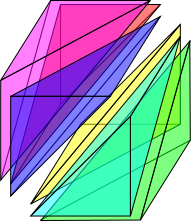
\includegraphics[width=.5\hsize]{kuhntriangulation.eps}
  \caption{\label{kuhntria}Kuhn triangulation in three dimensions.}
\end{figure}

\subsection{\label{kuhn}Kuhn Triangulation in a Nutshell}

Kuhn triangulation of the unit $n$-cube $[0, 1]^n$ is done by starting
in the origin $(0, \ldots, 0)$ and advancing by $1$ in direction of
the first dimension to the point $(1, 0, \ldots, 0)$, then by
advancing in direction of the second dimension by $1$ to the point
$(1, 1, 0, \ldots, 0)$ and so on until all dimensions have been
advanced by $1$ and point $(1, \ldots, 1)$ is reached.  All the $n+1$
points visited make up the corners of the first simplex of the
triangulation.  The other simplices are constructed in the same way,
the only difference is to permute the order in which the dimensions
are advanced.  Each permutation in the order of the dimensions
corresponds to exactly one member of the Kuhn triangulation and vice
versa.  Figure \ref{kuhntria} shows the resulting simplices of a Kuhn
triangulation in three dimensions.

\subsection{Terminology}

\begin{description}
\item[Kuhn simplex:] We call the members of a Kuhn triangulation we
  call {\em Kuhn simplices}.
\item[Kuhn0 simplex:] The Kuhn simplex corresponding to the identity
  permutation.
\item[size of a Kuhn simplex:] We define the size of a Kuhn simplex to
  be equal to its extension in direction $x_0$ (which is equal to its
  extension in the direction of any of the coordinate axes).
\end{description}

\subsection{Describing Kuhn Simplices by their Permutation}

We describe a simplex of size $s$ of a Kuhn triangulation in $n$
dimensions by the corresponding permutation $P$ of the vector
$\vec{v}:=(0,1,\ldots,n-1)$.  To get the coordinates of the corners
$\vec{x}_0,\ldots,\vec{x}_n$ of the simplex, we use the following
algorithm:
\begin{compactitem}
\item Let $\vec{p}:=P\vec{v}$.
\item Start at the origin $\vec{x}_0:=0$.
\item For each dimension $d$ from $0$ to $n-1$:
  \begin{compactitem}
  \item $\vec{x}_{d+1}:=\vec{x}_d+s\cdot\vec{e}_{p_d}$ ($\vec{e}_i$ is
    the unit vector in direction $i$.)
  \end{compactitem}
\end{compactitem}

\subsection{Index of a Permutation}

To give indices to the Kuhn simplices it is sufficient to index the
$n!$ permutations of $\vec{v}$.  All we need is a way to calculate the
permutation vector $\vec{p}$ of the permutation $P$ if given the
index.

$P$ can be made up of $n$ transpositions, $P=T_0\cdots T_{n-1}$.  Each
transposition $T_i$ exchanges some arbitrary element $t_i$ with the
element $i$, where $t_i\leq i$.  That means we can describe $P$ by the
integer vector $\vec{t}=(t_0,\cdots,t_{n-1})$, where $0\leq t_i\leq
i$.

Now we need to encode the vector $\vec{t}$ into a single number.  To
do that we take $t_i$ as digit $i$ of a number $p$ written in a ``base
faculty'' notation:
\[p=\sum_{i=1}^{n-1}i!t_i\]
This number $p$ is unique for each possible permutation $P$ so we
could use this as the index.  There is a problem though: we would like
the identity permutation $\vec{v}=P\vec{v}$ to have index 0.  So we
define the index $I$ of the permutation slightly differently:
\[I=\sum_{i=1}^{n-1}i!(i-t_i)\]
I can easily calculate the $t_i$ from $I$ ('/' denotes integer
division):
\[t_i=i-(I/i!)\bmod{(i+1)}\]

Note that $\vec{t}\not=\vec{p}$.  $\vec{t}$ obeys the relation
$t_i\leq i$, which is not necessarily true for $\vec{p}$.  To get
$\vec{p}$ we have to apply each $T_i$ in turn to $\vec{v}$.

\subsection{Number of Subvertices in a Kuhn0 Simplex}

Let $N(n,s)$ be the number of grid points within an $n$-dimensional
Kuhn0 simplex of size $s\in\mathbb{N}$ grid units.
The number of points in a $0$-dimensional simplex is $1$, independent of
its size:
\[N(0,s)=1\]
We slice the $n+1$ dimensional simplex orthogonal to one of the
dimensions and sum the number of points in the $n$-dimensional
sub-simplices.  This gives us the recursion formula
\[N(n+1,s)=\sum^s_{i=0}N(n,i)\;.\]
This formula is satisfied by the binomial coefficient\cite{bronstein}
\[N(n,s)=\left({n+s}\atop s\right).\]

Observations:
\begin{compactitem}
\item $N(n,0)=1$
\item $N(n,s)=N(s,n)$
\end{compactitem}

\begin{figure}
  \centering
  \includegraphics[width=.5\hsize]{simplexvertexindex.eps}
  \caption{\label{simplexindex}The image shows the Kuhn0 tetrahedron
    of width 2 (wire-frame).  It is partitioned into a tetrahedron
    (green), a triangle (red), a line (blue), and a vertex (black),
    each of size 1 and each a Kuhn0 simplex in its respective frame.}
\end{figure}

\subsection{Index of a Subvertex within a Kuhn0 Simplex}

Let $I(\vec{x})$ be the index of point $\vec{x}\in\mathbb{N}^n$ in the
$n$-dimensional Kuhn0 simplex of size $s$.  The coordinates measure
the position of the point in grid units and thus are integer.

Let us explain the idea in 3 dimensions (refer to figure
\ref{simplexindex}).  We want to calculate $I(2,1,1)$, which is 6
according to the figure.
\begin{itemize}
\item First we take the biggest tetrahedron not containing subvertex 6
  (which is the green tetrahedron in the figure) and count the number
  of vertices it contains, which gives us 4.  For the following we
  confine ourself to 2 dimensions by fixing $x_0=2$, which leaves us
  with a triangle consisting of the subvertices 4 to 9.
\item Now we count the number of vertices in the biggest triangle not
  containing subvertex 6.  The triangle consists solely of subvertex
  4, so the count is 1.  Again we confine ourself, this time to 1
  dimension be fixing $x_1=1$.  This leaves us with a line consisting
  of subvertices 5 and 6.
\item We count the subvertices in the biggest line not containing
  subvertex 6.  The line consist only of subvertex 5 so the count is 1
  again.  If we confine ourself any further we're left with 0
  dimensions, so we stop here.
\item We add the counted stuff together and get indeed 6.
\end{itemize}

This can easily be put into a formula.  We sum up all the vertices in
the sub-simplices not containing the point in question.  We know how to
count the subvertices from the previous section:
\[I(\vec{x})=\sum_{i=0}^{n-1}N(n-i,x_i-1)\]
Substituting $N$, we get
\[I(\vec{x})=\sum_{i=0}^{n-1}\left({n-i+x_i-1}\atop{n-i}\right)\]
Since the coordinates of a vertex within the Kuhn0 simplex obey the
relation $x_0\geq x_1\geq\cdots\geq x_{n-1}$, they cannot simply be
swapped so the sum is somewhat ugly.

\subsection{Number of Subelements in a Kuhn0 Simplex}

In $n$ dimensions, when we refine the $n$-dimensional hypercube of
size $s$ we get $s^n$ sub-hypercubes of size 1.  When we do a Kuhn
triangulation of the sub-hypercubes we get $n!$ sub-simplices for each
sub-hypercube, in total $s^n\cdot n!$ for the hypercube of size $s$.
When we triangulate this hypercube directly we get $n!$ Kuhn
simplices, each one of equal size, so each contains $s^n$ of the
sub-simplices.

\subsection{Index of a Subelement within a Kuhn0 Simplex}

We didn't come up with a way to simply map a subelement of a Kuhn0
simplex to an index number.  Luckily, the iterator interface only
requires that we are able to calculate the next subelement.

Each subelement is a Kuhn simplex which triangulates a hypercube.  We
need to remember the vertex which is the origin of that hypercube and
the index of the permutation that identifies the Kuhn sub-simplex.  Now
to get to the next subelement, we simply need to increment the
permutation index, and if it overflows we reset it and increment the
origin to the next vertex (we already know how to do that).

Some subelements generated this way are outside the refined Kuhn0
simplex, so we have to check for that, and skip them.

\begin{figure}
  \centering
  \includegraphics[width=.5\hsize]{referencetokuhn0.eps}
  \caption{\label{ref2kuhn0} Transforming Dunes reference simplex into
    the Kuhn0 simplex.  Step 1 moves each point by its $x_2$ value
    into $x_1$ direction.  Step 2 moves each point by its new $x_1$
    value into $x_0$ direction.}
\end{figure}

\subsection{Mapping between some Kuhn Simplex and the Reference Simplex}

Dunes reference simplex is defined as having one corner at the origin
and the others at 1 at each coordinate axis.  This does not match any
Kuhn simplex, but the transformation can be done quiet easily.

\subsubsection{Kuhn0 Simplex}

The algorithm to transform a point $\vec{x}=(x_0,\ldots,x_{n-1})$ from
the reference simplex of dimension $n$ to the Kuhn0 simplex (as
illustrated in figure \ref{ref2kuhn0}) is as follows:
\begin{compactitem}
\item For each dimension $d$ from $n-2$ down to 0:
  \begin{compactitem}
  \item $x_d:=x_d+x_{d+1}$.
  \end{compactitem}
\end{compactitem}\vspace{2ex}

The reverse (from Kuhn0 to reference) is simple as well:
\begin{compactitem}
\item For each dimension $d$ from 0 up to $n-2$:
  \begin{compactitem}
  \item $x_d:=x_d-x_{d+1}$.
  \end{compactitem}
\end{compactitem}

\subsubsection{Arbitrary Kuhn Simplices}

For arbitrary Kuhn simplices we have to take the permutation of that
simplex into account.  So to map from the reference simplex of $n$
dimensions to the Kuhn simplex with the permutation $P$ (which is
described by the vector $\vec{p}=P(0,\ldots,n-1)$) we do:
\begin{compactitem}
\item For each dimension $d$ from $n-2$ down to 0:
  \begin{compactitem}
  \item $x_{p_d}:=x_{p_d}+x_{p_{d+1}}$.
  \end{compactitem}
\end{compactitem}\vspace{2ex}

And for the reverse:
\begin{compactitem}
\item For each dimension $d$ from 0 up to $n-2$:
  \begin{compactitem}
  \item $x_{p_d}:=x_{p_d}-x_{p_{d+1}}$.
  \end{compactitem}
\end{compactitem}

\begin{thebibliography}{0}
\bibitem{dune} Distributed and Unified Numerics Environment
  \url{http://www.dune-project.org}.
\bibitem{jbey} J\"urgen Bey: ``Finite-Volumen-
    und Mehrgitterverfahren f\"ur elliptische Randwertprobleme.''  The
  relevant part is available in english at
  \url{http://www.igpm.rwth-aachen.de/bey/ftp/simplex.ps.gz}.
\bibitem{bronstein} Bronstein, Semendjajew, Musiol, M\"uhlig
  ``Taschenbuch der Mathematik'' (1999)

\end{thebibliography}

\end{document}
